\chapter{Experimental Infrastructure}

In this section, the hardware and frameworks used for this thesis will be described. The hardware used was mainly the ATLASCAR 2 and its sensors: two SICK LMS151 \gls{lidar}, one SICK LD-MRS \gls{lidar} and a PointGrey Zebra 2 Camera. The central framework that receives messages from the sensors is \gls{ros}. This data will be processed using the \gls{opencv} for images, and several libraries will be used for the range-based sensors, such as the \gls{pcl} and \gls{mtt}. 

\section{ATLASCAR 2}

The ATLASCAR 2 is based in the platform of the 2015 Mitsubishi i-MiEV, a full electric vehicle. The battery that powers the engine is the same powering the camera and the sensors. The main characteristics of the car are in table \ref{tab: MiEV technical} (\cite{MITSUBISHIMOTORS}). 

\begin{figure}[htp]
	
	\centering
	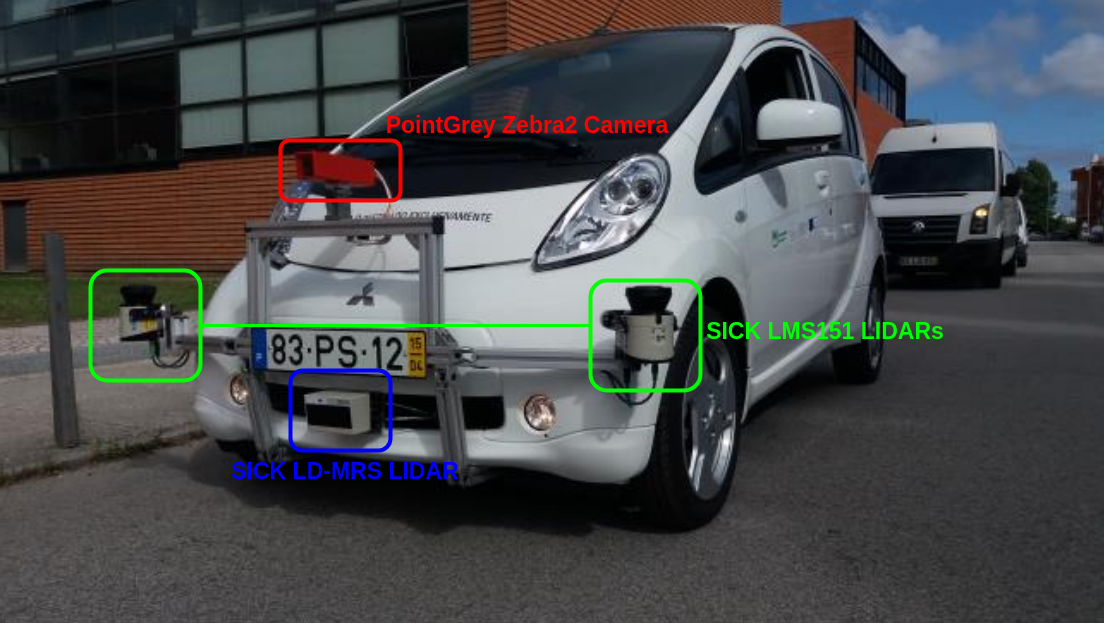
\includegraphics[width=.9\textwidth]{capexp/imgs/atlascar2.png}\hfill
	
	\caption{The ATLASCAR 2 based on the Mitsubishi i-MiEV platform equipped with a camera and several LIDAR sensors}
	\label{fig:imiev}
	
\end{figure}

\begin{table}[!h]
	\centering
	\caption{Mitsubishi i-MiEV technical specifications}
	\label{tab: MiEV technical}
	\begin{tabular}{lcc}
		Characteristic & Unit & Value\\
		Wheelbase & mm & 2550\\
		Track (Front/Rear) & mm & 1310/1270 \\
		Vehicle weight & kg  & 1450 \\
		\hline
		Engine & -- & Electric \\
		Electric energy consumption & Wh/km & 135 \\
		Electric range (NEDC)  & km & 150 \\
		Maximum speed & km/h & 130 \\
		Minimum turning radius & m & 4.5 \\
		Max. Power output & kW & 49 \\
		Max. torque & Nm & 180 \\
		\hline
		Traction battery type & -- & Lithium-ion battery \\
		Traction battery voltage & V & 330 \\
		Traction battery energy & kWh & 16 \\
		Regular charging (AC 230V 1 phase) 8A & hrs & 10 \\
	\end{tabular}
\end{table}

\section{Sensors}

The sensors equipped in the ATLASCAR 2 are two SICK LMS151 \gls{lidar}, a SICK LD-MRS \gls{lidar} and a PointGrey Zebra 2 Camera. It is of most importance for the ATLASCAR 2 to have this sensors to be capable of perception. The sensors have been mounted in the front of the car in an aluminum infrastructure designed by \cite{Correia2017}. These devices are connected to a network switch installed in the car to which a computed can be plugged to receive the data from the sensors.

\subsection{SICK LMS151 LIDAR}

The SICK LMS151 (figure \ref{fig:sicklms}) is a \gls{lidar} sensor designed to be used in outdoors. It is a planar infrared scanner with a large planar aperture angle often used in robotics and in \gls{ad} fields for its high scanning frequency and operating range. This scanner is also able to scan distances through fog, glass and dust (multi-echo technology). This scanner is provided with an Ethernet TCP/IP interface with high data transmission rate. \cite{SICK}

\begin{figure}[htp]
	
	\centering
	\hfill
	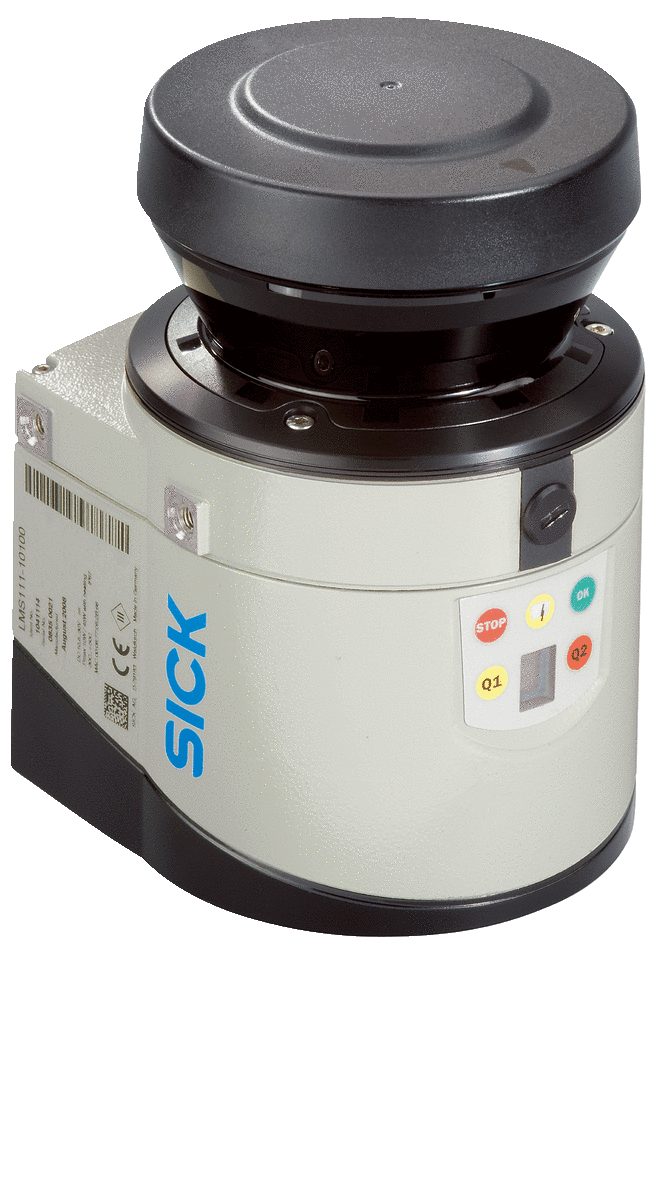
\includegraphics[width=.3\textwidth]{capexp/imgs/sicklms}\hfill
	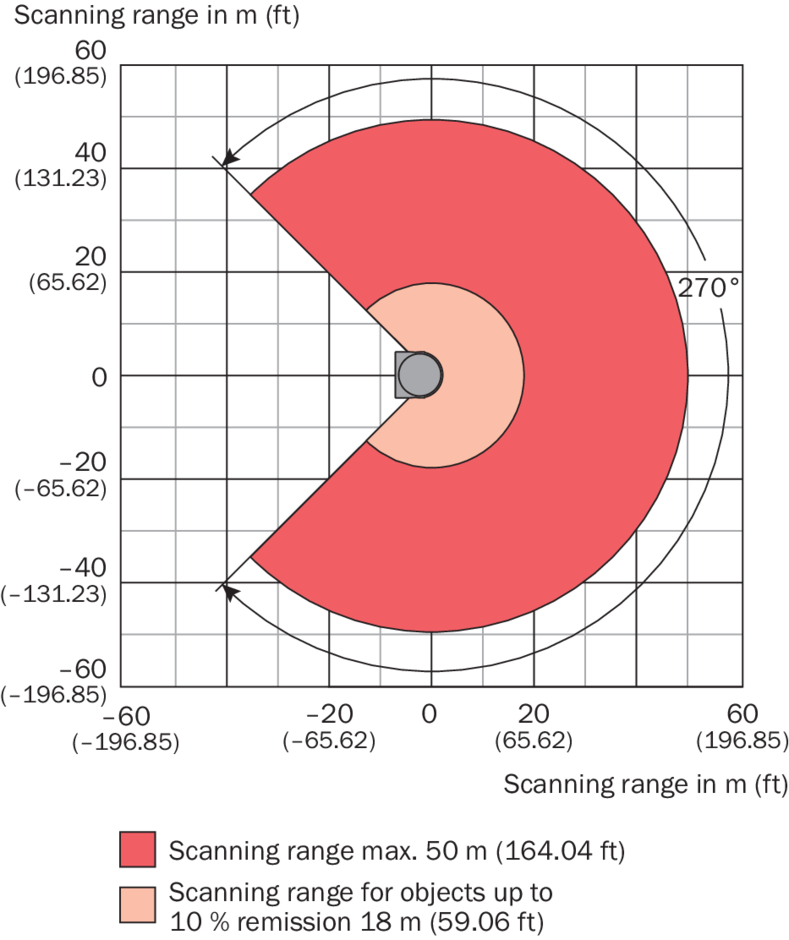
\includegraphics[width=.5\textwidth]{capexp/imgs/sicklms2}\hfill
	
	\caption{The SICK LMS151 LIDAR and its operating range}
	\label{fig:sicklms}
	
\end{figure}

\begin{table}[!h]
	\centering
	\caption{SICK LMS151 specifications}
	\label{tab: sicklmsspecs}
	\begin{tabular}{ll}
		\hline
		Field of application & Outdoors\\
		Laser Class & 	1 (IEC 60825-1:2014, EN 60825-1:2014) \\
		Aperture Angle & 270$^{\circ}$ \\
		Scanning frequency & 25 Hz / 50 Hz \\
		Angular resolution	& 0.25$^{\circ}$ / 0.5$^{\circ}$ \\
		Operating range	& 0.5 m ... 50 m \\
		Max. range with 10 \% reflectivity & 18 m \\
		Amount of evaluated echoes & 2 \\
		Data transmission rate & 10/100 MBit/s \\
		\hline
	\end{tabular}
\end{table}

For this project, the SICK LMS151 will operate at 50 Hz with an angle increment of 0.5$^{\circ}$ between readings. Each message will transmit a total of 540 points per scan in polar coordinates $(r,\theta)$. \cite{SICK}

\subsection{SICK LD-MRS LIDAR}

The SICK LD-MRS (figure \ref{fig:sickldmrs}) is a \gls{lidar} sensor also designed to be used in outdoors. It features 4 planar infrared scanners with 0.8$^{\circ}$ vertical aperture angle between each plan, offering tri-dimensional point clouds. It provides high scanning frequencies and long operating range up to 300 meters. This scanner is also provided with an Ethernet TCP/IP interface with high data transmission rate (\cite{SICKa}).

\begin{figure}[htp]
	
	\centering
	\hfill
	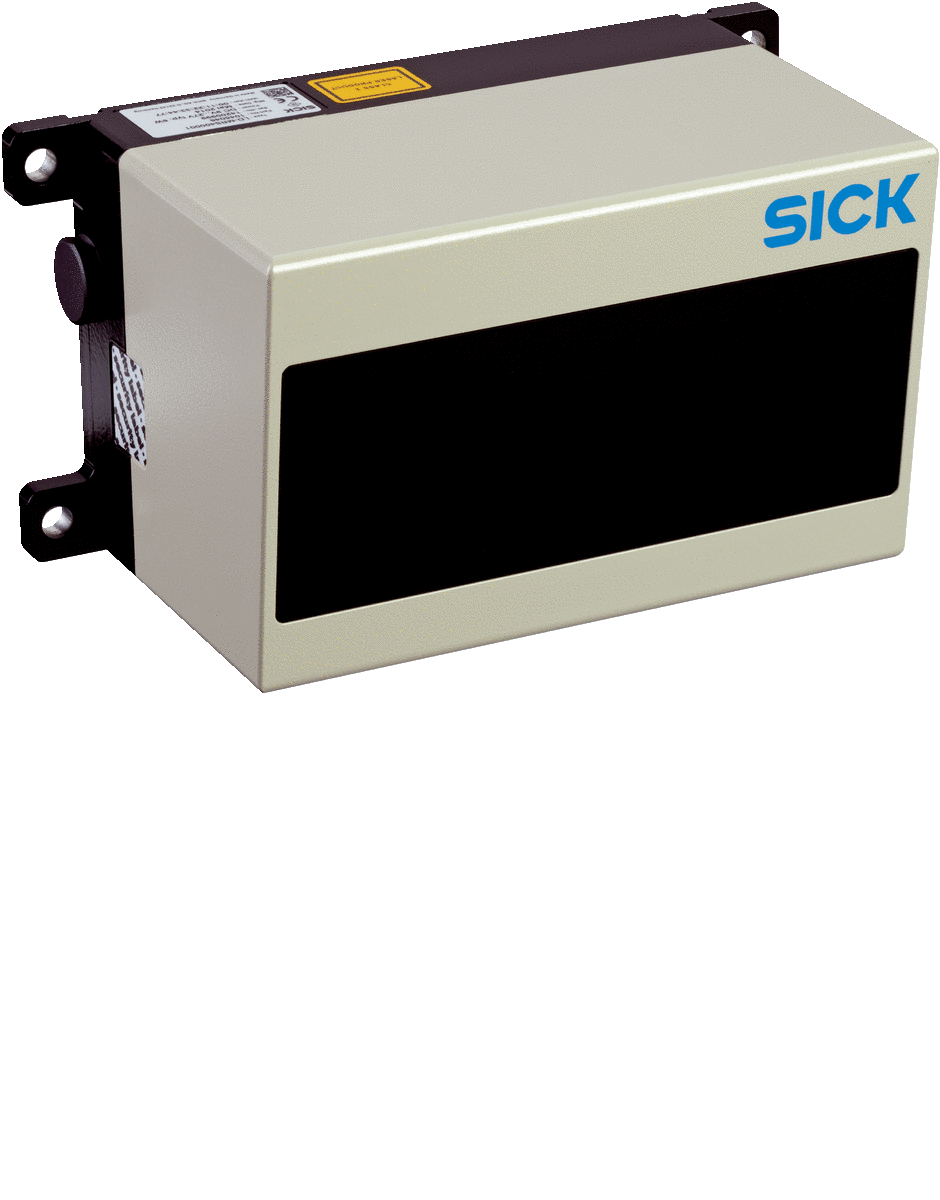
\includegraphics[width=.4\textwidth]{capexp/imgs/sickldmrs}\hfill
	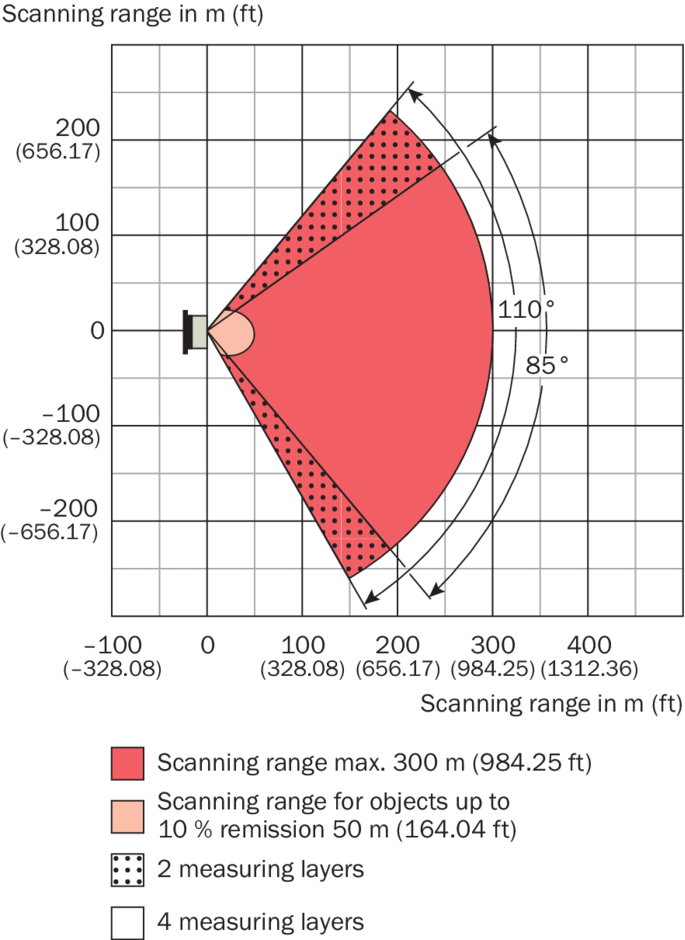
\includegraphics[width=.5\textwidth]{capexp/imgs/sickldmrs2}\hfill
	
	\caption{The SICK LD-MRS LIDAR and its operating range}
	\label{fig:sickldmrs}
	
\end{figure}

\begin{table}[!h]
	\centering
	\caption{SICK LMS151 specifications}
	\label{tab: sickldmrsspecs}
	\begin{tabular}{ll}
		\hline
		Field of application & Outdoors\\
		Laser Class & 	1 (IEC 60825-1:2014, EN 60825-1:2014) \\
		Scanner Planes & 4 measuring planes \\
		Aperture Angle & 85$^{\circ}$  \\
		Total Aperture & 110$^{\circ}$\\
		Scanning frequency & 12.5 Hz / 50 Hz \\
		Angular resolution	& 0.125$^{\circ}$ / 0.25$^{\circ}$ / 0.5$^{\circ}$ \\
		Operating range	& 0.5 m ... 300 m \\
		Max. range with 10 \% reflectivity & 50 m \\
		Amount of evaluated echoes & 3 \\
		Data transmission rate & 100 MBit/s \\
		\hline
	\end{tabular}
\end{table}

For this project, the SICK LD-MRS will operate at 50 Hz with an angle increment of 0.5$^{\circ}$ between readings. Each message will transmit a total of 200 points per scan in polar coordinates $(r,\theta)$ for each plan. Since this scanner offers four planar scans, the final point cloud will total 800 points (\cite{SICKa}).

\subsection{PointGrey Zebra 2 Camera}

The PointGrey Zebra 2 Camera (figure \ref{fig:pointgrey}) is a high resolution camera with a Sony ICX274. It also features a GigE PoE Interface and it is highly configurable to fulfill any particular utilization needs (\cite{PointGrey}). The camera is inserted in a case made with 3D printing and designed by \cite{Correia2017}.  Other relevant specifications are found in table \ref{tab: pointgreyspecs}. 

\begin{figure}[htp]
	
	\centering
	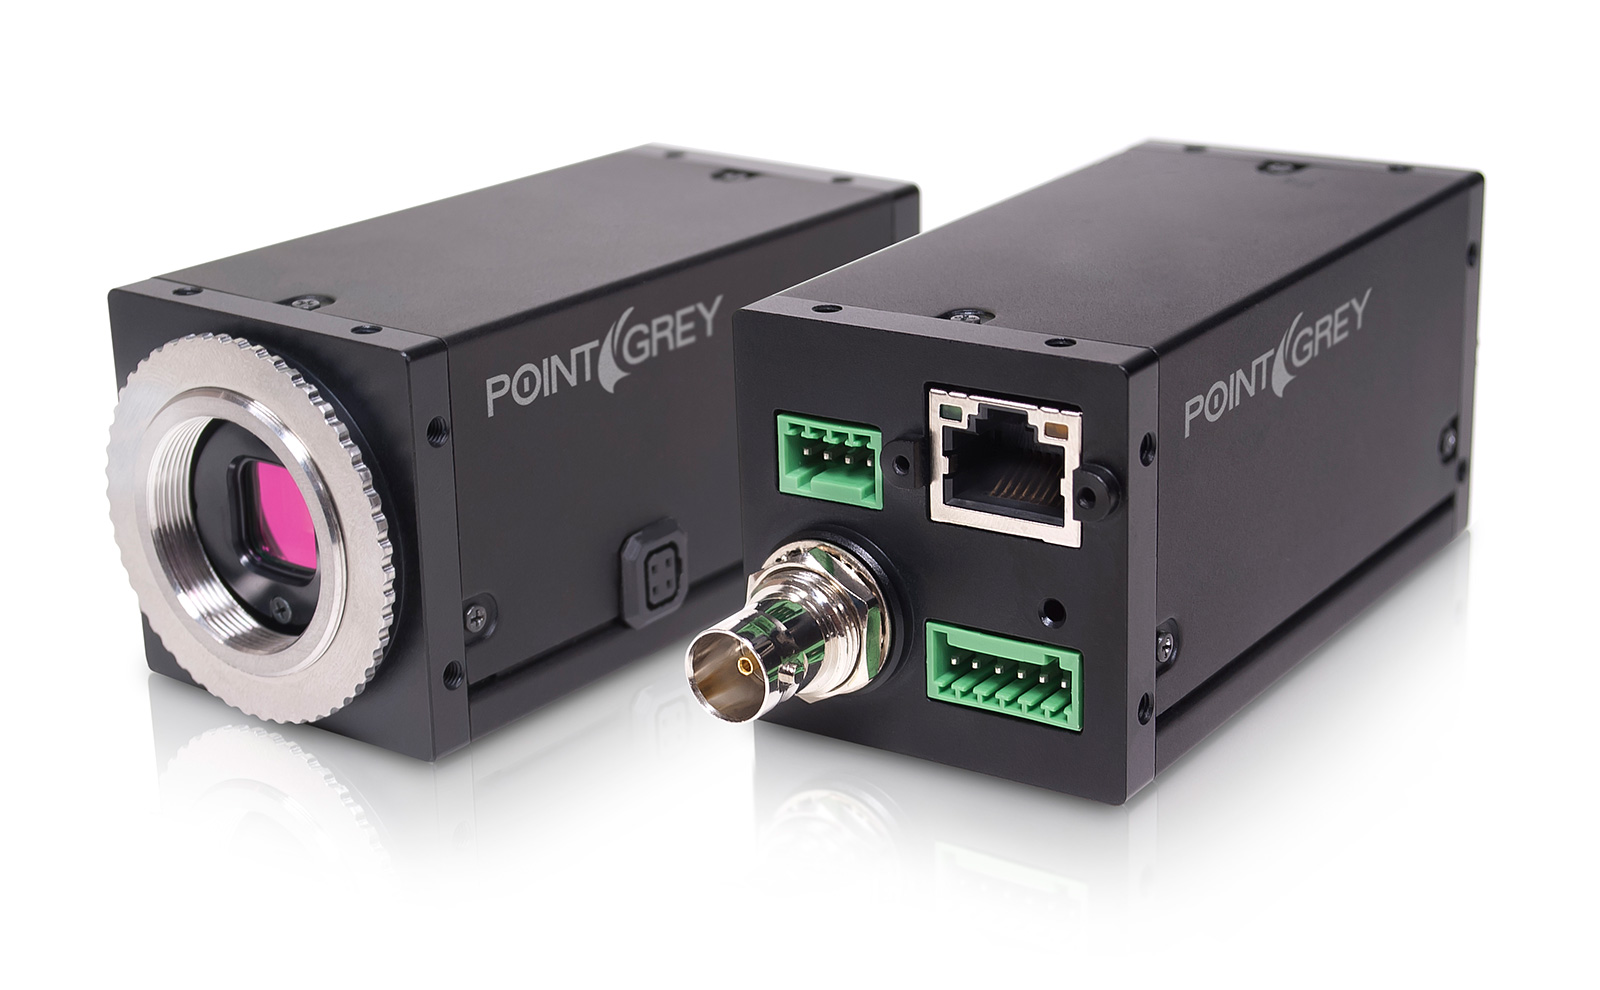
\includegraphics[width=.6\textwidth]{capexp/imgs/pointgrey}
	
	\caption{The PointGrey Zebra 2 Camera}
	\label{fig:pointgrey}
	
\end{figure}

\begin{table}[!h]
	\centering
	\caption{PointGrey Zebra 2 Camera specifications}
	\label{tab: pointgreyspecs}
	\begin{tabular}{ll}
		
		\hline
		Resolution & 1624 x 1224\\
		Max. Frame Rate & 25 FPS with HD-SDI \\
		Megapixels & 2.0 MP \\
		Chroma & Color\\
		Sensor & Sony ICX274 CCD \\
		Image Buffer &	32 MB\\
		Interface &	GigE PoE, HD-SDI\\
		
		\hline
	\end{tabular}
\end{table}

Working at maximum resolution and frame rate would saturate the network bandwidth and increase image processing times. In this project the camera's frame rate is set at 7.5 FPS so that a balance between image quality and processing optimization can be accomplished.


\section{Software}

In this section it will be discussed the software used in this dissertation. The base architecture of this dissertation is centered in the \gls{ros} framework. Many \gls{ros} tools and features are used such as Rviz, rosbags, roslaunch and rosrun. Two main nodes are to be developed in this work: the camera calibration package node (previously developed by \cite{VieiradaSilva2016}) and the labelling node. The handling of data from the sensors was done using \gls{pcl}, \gls{mtt}, 
and the image processing was performed with \gls{opencv} libs. All software was programmed with C++.

\section{ROS}
The central framework in the ATLASCAR 2 is based on \gls{ros} Kinect on Ubuntu 16.04.

The Robot Operative System, although not an operating system, operates as a robotics middleware. \gls{ros} offers open-source services designed for developers that need hardware abstraction and low-level device control. Architectures in \gls{ros} are centered in applications called rosnodes which communicate with each other creating a graph of  message-passing processes. 

With \gls{ros} it is possible to receive data packets and transform them in messages that contain data from the sensors. It is possible to manipulate this data using \gls{ros} nodes and other tools. 

\subsection{Rviz}
Rviz is the standard \gls{ros} tool for 3D visualization. %falar mais um pouco sobre o rviz%

The Rviz is one of the most important tools as it will be used to visualize data from the ATLASCAR 2 either directly in real-time by connecting a computer to the car or in rosbags. It will also serve as a debugging tool in which pointcloud values can be analyzed (\cite{ROSWiki}).

\subsection{Rosbag}

A rosbag is a file in \gls{ros} which contains messages saved from past events. While connected directly to a device, or several devices, multiple topics can be subscribed at once to be recorded into a rosbag. 

The advantage of rosbags in this dissertation is to simulate the working environment of the ATLASCAR 2 without actually being in it. Several rosbags were recorded throughout the process of development in this project, either of calibration or for detection, tracking and labeling purposes. 

In \gls{ros}, the rosbag package contains a set of tools for recording from and playing back to \gls{ros} topics. It is intended to be high performance and avoid deserialization and reserialization of the messages. It also features command line tools for working with bags as well as code APIs to read/write and manipulate bags (\cite{ROSWikia}).

\subsection{Roslaunch}
The roslaunch files are used as a tool for easily launching multiple \gls{ros} nodes. A roslaunch file sets up a roscore (os \gls{ros} master), sets parameters on the Parameter Server, and can also execute other roslaunch files. 

It includes options to automatically re-spawn processes that have already died. The roslaunch takes in one or more XML configuration files (with the .launch extension) that specify the parameters to set and nodes to launch.

For example, a rosbag can be given as parameter to the roslaunch which opens the Rviz with a previous defined configuration to visualize the data from that rosbag.

In this project, roslaunch files are optimal to set up calibration values before launching the Rviz and the nodes that process the data from the \gls{lidar}s and the camera. The transformations between device frames are set up using roslaunch files and static transform publishers implemented by \gls{ros}. 

The roslaunch files are also advantageous to set up the multiple drivers needed to bring up the several devices equipped in the ATLASCAR 2. Since the sensors are connected to a network switch, the parameters given in the driver's roslaunch file are the IP addresses of each of the devices. The drivers will then receive packets from the sensors and remap them into the \gls{ros} format.

\section{LAR Toolkit}

The \gls{lartk} is a software suite developed by members of the \gls{lar}. The projects involved in the \gls{lartk} are based in the development of robotic solutions namely for the ATLAS project. The toolkit is constituted by a set of packages, in which 2 main packages will be used for this disseration: the multi-sensor calibration package and the \gls{mtt} package.

\subsection{Multi-sensor calibration package}

The multi-sensor calibration package is a package developed by \cite{VieiradaSilva2016}. The package contains a \gls{gui} used to calibrate the several sensors in the ATLASCAR 2. The package was initially developed for the ATLASCAR 1, and it was further used into the ATLASCAR 2 since the sensors were almost the same.

The calibration package features a graphical user interface in which several sensors can be selected to be calibrated. The available devices are the SICK LMS151 and SICK LD-MRS mounted in the ATLASCAR 2, PointGrey cameras, Microsoft Kinects, the SwissRanger SR4000 and the Velodyne VLP16 used in the ATLASCAR 1.


\subsection{Multi Target Tracking (MTT)}

The \gls{mtt} library is a set of methods and strategies developed by \cite{SoaresDeAlmeida2016a} specially designed for the ATLASCAR project with the goals to use the planar scanners to obtain perception about objects captured in the \gls{lidar}s. The ATLASCAR2 is equipped with scanners that send data in a message format. 

The \gls{mtt} is capable of receiving these messages and break them in smaller groups. This process is called clustering. Clustering separates all objects found in a scan and returns their position. The clustering of data is an important step in the development of this dissertation as it facilitates the detection and tracking of objects in space. 

The clustering algorithm of the \gls{mtt} library segments the received pointclouds using a predefined distance as threshold. Each set of points in the clusters are assumed as possible targets of interest.

The \gls{mtt} then associates the targets found to a linked list of objects where the full description of the objects are stored. This list is later used to create a motion model where the estimated position of the objects and its velocity is calculated. 

Some objects may become occluded, for example when a car passes in front of another. The \gls{mtt} estimates the position of the occluded objects by creating a motion model using their velocity and so it is possible to track objects while they are out of the field of view but still in the surroundings.

The \gls{mtt} operates around targets. Targets keep information about the object and its velocity plus their position and obstacle lines.

\section{\gls{pcl}}

The \gls{pcl} is a library that implements methods to process pointcloud data. The \gls{pcl} framework contains numerous state of the art algorithms including filtering, feature estimation, surface reconstruction, registration, model fitting and segmentation (\cite{PointCloudLibrary2018}). Some of these algorithms are used throughout this thesis an were also used by the \gls{mtt} library.
It is important to use the \gls{pcl} in this project as it works with a lot of data from \gls{lidar} sensors at the same time. 



 








